\documentclass[a4paper,12pt]{article}
\usepackage[latin1]{inputenc}
\usepackage[spanish]{babel}
\usepackage{amsmath}
\usepackage{graphicx}
\setlength{\textheight}{250mm}
\setlength{\textwidth}{165mm}
\setlength{\topmargin}{-15mm}
\setlength{\oddsidemargin}{0pt}
\pagestyle{empty}

\begin{document}

\def\bm#1{{\mbox{\boldmath $#1$}}}
\def\eqdef{\buildrel \rm def \over =}
\def\signo{\mathop{\rm signo}\nolimits}

\mbox{}\vspace*{-20mm}

{\centering
{\small\sc Escuela Técnica Superior de Ingenieros de Caminos, Canales y Puertos (Madrid)}\\*[4mm]
{\Large\bf Método de los Elementos Finitos (Curso 18-19)}\\*[4mm]
EJERCICIO 4: Tecnología de elementos.
}

% \vspace{4mm}

% ENUNCIADO
La estructura de la figura, cuyas dimensiones están indicadas en la misma,
está fabricada con un material cuyas propiedades mecánicas son
$E=20.5$ GPa y $\nu=0.23$. Las cargas aplicadas tienen todas el mismo
valor $F=1000$ kN. Las condiciones de contorno a aplicar son las
correspondientes a que los planos $OXY$, $OXZ$ y $OYZ$ sean planos de
simetría.

La discretización a considerar son $3$ elementos en el espesor y $20x20$
elementos en las caras verticales (situadas fuera de los planos
coordenados). Para resolver el problema se utilizarán elementos hexaédricos
de $8$ nodos con formulaciones en desplazamientos, mixta y
deformaciones mejoradas supuestas (modos incompatibles).

\vspace{5mm}
\begin{center}
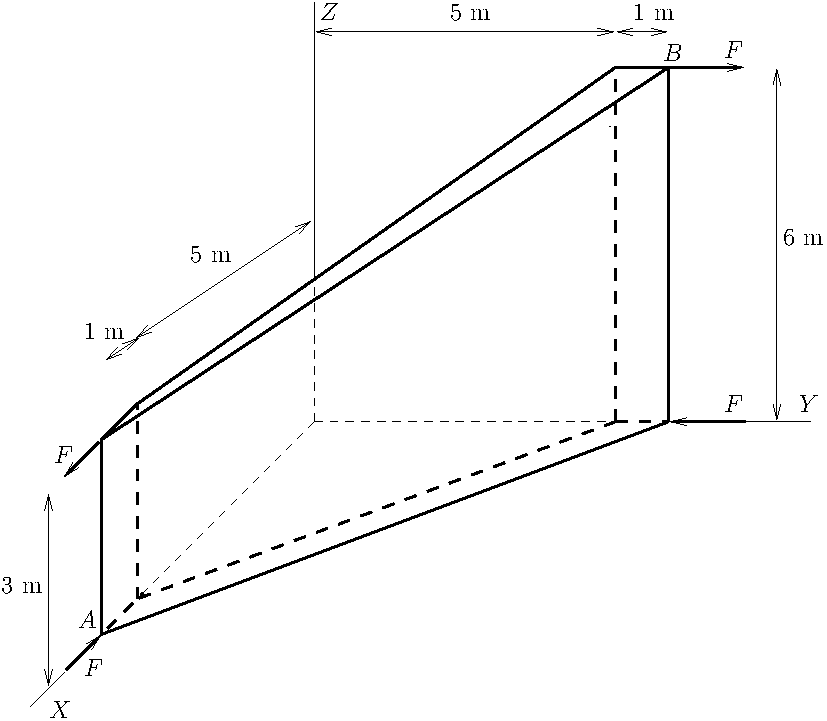
\includegraphics[width=0.7\textwidth]{ejerc4}
\end{center}

\end{document}
